

\documentclass{sig-alternate-05-2015}

% Include useful packages
\usepackage{graphicx}
\graphicspath{ {images/} }
\usepackage{float}


\begin{document}

% Copyright
\setcopyright{acmcopyright}


\title{Testing and Tuning SkinnyDip: Noise-Robust Clustering}
\numberofauthors{2} 
\author{
% You can go ahead and credit any number of authors here,
% e.g. one 'row of three' or two rows (consisting of one row of three
% and a second row of one, two or three).
%
% The command \alignauthor (no curly braces needed) should
% precede each author name, affiliation/snail-mail address and
% e-mail address. Additionally, tag each line of
% affiliation/address with \affaddr, and tag the
% e-mail address with \email.
%
% 1st. author
\alignauthor
Grant King\\
       \email{kinggra1@msu.edu}
}
% There's nothing stopping you putting the seventh, eighth, etc.
% author on the opening page (as the 'third row') but we ask,
% for aesthetic reasons that you place these 'additional authors'
% in the \additional authors block, viz.
\date{17 February 2017}
% Just remember to make sure that the TOTAL number of authors
% is the number that will appear on the first page PLUS the
% number that will appear in the \additionalauthors section.

\maketitle

\begin{figure*}[t]
\centering
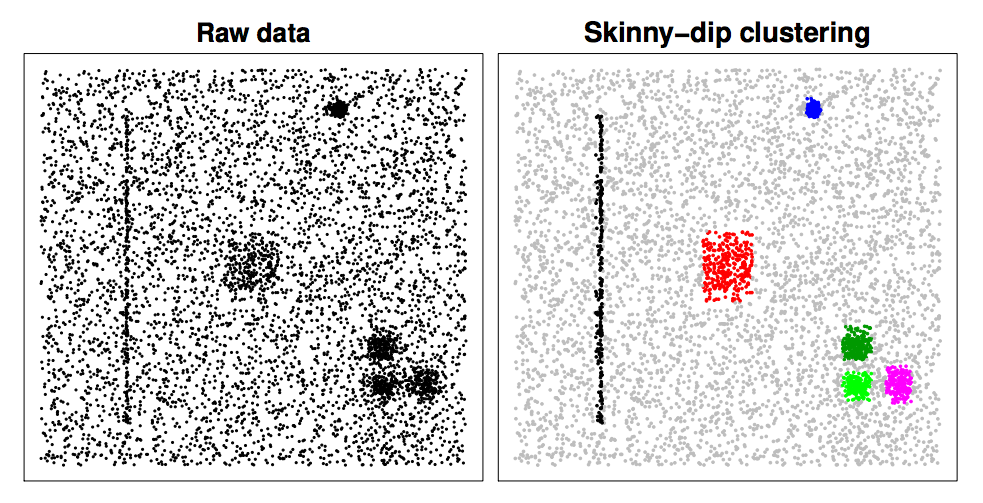
\includegraphics[width=\textwidth]{images/SkinnyDipExample}
\caption{The running example used by Maurus, et al. throughout \cite{skinnydip}}
\label{fig:algor}
\end{figure*}

\section{Problem Description}
It is not uncommon for some real-world data sets to feature an abundance of noise. Depending on the severity of this noise, classical clustering methods may fail due to due to dependence on clean data or confusion from increasingly excessive noise. SkinnyDip is an algorithm proposed by Maurus et al.\cite{skinnydip} designed to handle clustering data in highly noisy environments. SkinnyDip is based on the statistical concept of the \textit{dip} \cite{dip}. 

The dip views the structure of the Empirical Cumulative Distribution Function(ECDF) of a set of single dimensional data to determine whether it is unimodal or multimodal. This test is expanded to a multidimensional, recursive heuristic in order to isolate the various modes of each feature of a set of data. This results in a deterministic, parameter-free, unsupervised method of finding clusters that are based on the modes of multivariate distributions. 

A visual example of the purpose of SkinnyDip is demonstrated in the running example from \cite{skinnydip} which shows the extraction of distinct shapes from a two-dimensional data field that consists of 80\% static noise. A variety of similar clustering methods were shown to perform poorly on this data set, both through the inclusion of the evenly-distributed, static noise in clusters, and through over-segmentation of the existing classes.

My goal is to implement the SkinnyDip algorithm and perform additional tests to demonstrate its usefulness on noisy, real-world data sets, with a final goal of reducing the extraneous information introduced by SkinnyDip's hypercubic boundaries through extension with a second clustering method.


\section{Related Work}
Data clustering is a fundamental problem in Machine Learning, and has been approached in a variety of ways, resulting in a plethora of tools and methods \cite{ClusteringMethods}, many of which are sensitive to noise and other outliers. Additionally, many common techniques, such as k-means clustering, operate as closed set clustering methods and are unable to reject noise at all.

\cite{DBSCAN} is a density-based technique for finding clusters in environments that may contain noise. However, it has the disadvantages of being a parameterized method, and still continues to find extraneous clusters in increasingly noisy data when compared to SkinnyDip.

A single other existing method for clustering using the statistical dip test was found, a technique called DipMeans\cite{dipmeans}. This method, however, takes a different approach to the test, and performs the dip test on a collection of distance measurements as opposed to the raw data values themselves. SkinnyDip, however, requires no distance measurements  and is both functionally and computationally distinct from the DipMeans technique.


\begin{figure*}[t]
\centering
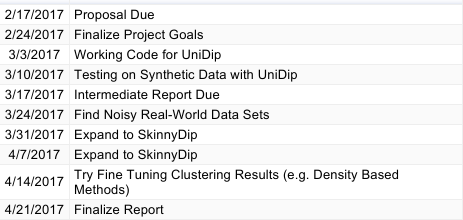
\includegraphics[width=\textwidth]{images/timeline}
\caption{Tentative Project Milestones}
\label{fig:milestones}
\end{figure*}

\section{Project Milestones}
Projected Project Milestones are given in \ref{fig:milestones}. It appears that most of the work will be in creating an actual implementation of the SkinnyDip algorithm itself in MATLAB. This may be mitigated by using an existing code base implemented in R and focusing more on the testing and extension vs. the algorithm itself, though this would require the extra learning curve of an entirely new language and tool set. Beyond this, the work that will largely be reported for this project will involve working with some real-world data (currently considering star data and galaxy clustering) as well as testing methods to improve the accuracy of SkinnyDip under higher-dimensional data sets.
\bibliography{proj-proposal}
\bibliographystyle{unsrt}
\end{document}
